\documentclass[conf]{new-aiaa}
%\documentclass[journal]{new-aiaa} for journal papers
\usepackage[utf8]{inputenc}

\usepackage{graphicx}
\usepackage{amsmath}
\usepackage[version=4]{mhchem}
\usepackage{siunitx}
\usepackage{subcaption}
\usepackage{longtable,tabularx}
\setlength\LTleft{0pt} 

\title{Open-Vocabulary Obstruction Detection for UAS Landing via Fine-Tuned YOLO-World}

\author{Andre Arante\footnote{Undergraduate Research Assistant, Department of Electrical and Computer Engineering, Washington DC, and AIAA Student Member.}, Mahyar Ghazanfari\footnote{Ph.D. Student, Department of Mechanical and Aerospace Engineering, George Washington University, AIAA Student Member.}, Can Vu\footnote{Ph.D. Student, Department of Mechanical and Aerospace Engineering, George Washington University, AIAA Student Member.}, and Peng Wei\footnote{Associate Professor, Department of Mechanical and Aerospace Engineering, George Washington University, AIAA Associate Fellow.
}}
\affil{George Washington University, Washington, DC, 20052}

% \author{Third C. Author\footnote{Insert Job Title, Department Name, Address/Mail Stop, and AIAA Member Grade (if any) for third author.}}
% \affil{Business or Academic Affiliation 2, City, Province, Zip Code, Country}
% \author{Fourth D. Author\footnote{Insert Job Title, Department Name, Address/Mail Stop, and AIAA Member Grade (if any) for fourth author (etc.).}}
% \affil{Business or Academic Affiliation 2, City, State, Zip Code}

\begin{document}

\maketitle

% Abstract
\begin{abstract}
Safe autonomous landing remains a critical challenge for unmanned aerial systems (UAS) performing package delivery, where undetected landing zone obstructions pose significant dangers. Traditional closed-set object detectors cannot generalize to arbitrary obstacles outside their training distribution, making them insufficient for real-world deployment. This paper investigates the tradeoff between domain-specific accuracy and open-vocabulary retention when fine-tuning YOLO-World, a real-time open-vocabulary object detection model, on the VisDrone aerial dataset for UAS landing zone obstruction detection. The CLIP text encoder is frozen during fine-tuning to mitigate open-vocabulary degradation, restricting weight updates to the detection head and neck. Experiments across three training durations (5, 40, and 80 epochs) demonstrate that 
extended fine-tuning increasingly biases the model toward VisDrone-specific classes at the cost of open-vocabulary responsiveness, while a 5-epoch checkpoint achieves the strongest balance (mAP@0.5: 0.492, +149\% over baseline, while retaining open-vocabulary capabilities). Real-time inference is demonstrated on NVIDIA Jetson Xavier and Jetson Orin Nano embedded platforms, confirming practical feasibility for onboard UAS deployment.
\end{abstract}

\section{Introduction}

The rapid expansion of unmanned aerial system 
(UAS) operations in commercial logistics has positioned 
autonomous package delivery as a near-term reality for 
last-mile supply chains. Major operators such as 
Zipline~\cite{zipline2025} and Wing~\cite{wing2025} have 
already received FAA approval for beyond-visual-line-of-sight 
(BVLOS) commercial operations, while companies including 
Amazon, DHL, and FedEx continue to develop UAS logistics 
at scale.\cite{marquand2023faa, zieher2024drones} Despite 
this momentum, safe autonomous landing remains one of the 
most operationally significant unsolved challenges in the 
field. The landing phase requires the UAS to localize the 
landing zone and verify it is clear of obstructions, a 
task made particularly difficult in dynamic last-mile 
environments such as residential driveways and front yards, 
where hazards range from stationary obstacles such as 
vehicles and debris to dynamic ones such as pedestrians 
and pets \cite{alam2023survey}.

Previous landing systems rely on traditional closed-set object detectors such as YOLOv8 \cite{ultralytics2023} to recognize the marker from drone-mounted cameras \cite{fattahi2017automatic, xu2024small}. While effective for marker localization, these detectors cannot generalize beyond their training categories, making them fundamentally insufficient for safe autonomous landing.

Open-vocabulary object detection (OVOD) offers a promising alternative. YOLO-World integrates a CLIP-based text encoder into the real-time YOLO framework, enabling detection of arbitrary object categories specified through natural language prompts at inference time \cite{cheng2024yoloworld, radford2021learning}. However, deploying YOLO-World on UAS hardware requires fine-tuning on aerial datasets to close the domain gap between ground-level pretraining data and top-down drone imagery. It has been observed that fine-tuning the CLIP encoder on domain-specific data leads to severe degradation of open-vocabulary generalization, the very capability that motivates its use \cite{cheng2024yoloworld}. Navigating this tradeoff is the central challenge this paper addresses.

This paper makes the following contributions. First, we present a fine-tuning methodology for YOLO-World on the VisDrone dataset that freezes the text encoder during training, preserving open-vocabulary generalization, and evaluates checkpoints at three training durations to empirically characterize the specialization-retention tradeoff. Second, we investigate whether descriptive noun phrase prompts such as ``foreign object on orange circle landing pad'' can detect novel obstructions not explicitly prompted for at inference time. Third, we evaluate the fine-tuned model for real-time inference on NVIDIA Jetson Xavier and Jetson Orin Nano embedded platforms, demonstrating practical feasibility for onboard UAS deployment.

\section{Related Works}

\subsection{Traditional Object Detection}

One approach to the problem of autonomous UAS landing has been 
through marker-based detection systems in which an ArUco marker 
is placed at the landing site and detected by an onboard camera 
during descent. These markers encode a unique binary pattern 
that can be detected and decoded in real time using classical 
computer vision techniques, allowing the UAS to estimate its 
position and orientation relative to the landing zone with high 
precision (Fig.~\ref{fig:aruco}) \cite{fattahi2017automatic}. 
However, marker-based approaches carry one significant 
limitation: they require consumers to correctly place the 
marker at a landing site in advance.

In contrast, approaches have been proposed to address this 
limitation. The Obstacle and Landing Site Awareness System 
(OLSAS)~\cite{xu2024small} demonstrated the feasibility 
of detecting a generic landing pad (Fig.~\ref{fig:landingpad}) from drone-mounted cameras without relying on ArUco markers, supporting 
safe autonomous package delivery landings. These approaches 
demonstrate that deep learning based landing site detection 
is viable, but struggle with the fundamental limitation of 
traditional closed-set detection methods: the models are 
trained on a fixed list of object categories and cannot 
generalize to novel obstructions not present in the training 
data. 


\begin{figure}[hbt!]
\centering
\begin{subfigure}{0.45\textwidth}
    \centering
    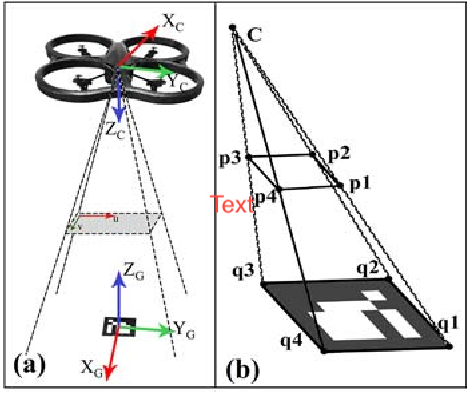
\includegraphics[height=4cm, keepaspectratio]{aruco_landing_pad.png}
    \caption{ArUco marker used in prior landing systems.}
    \label{fig:aruco}
\end{subfigure}
\hfill
\begin{subfigure}{0.45\textwidth}
    \centering
    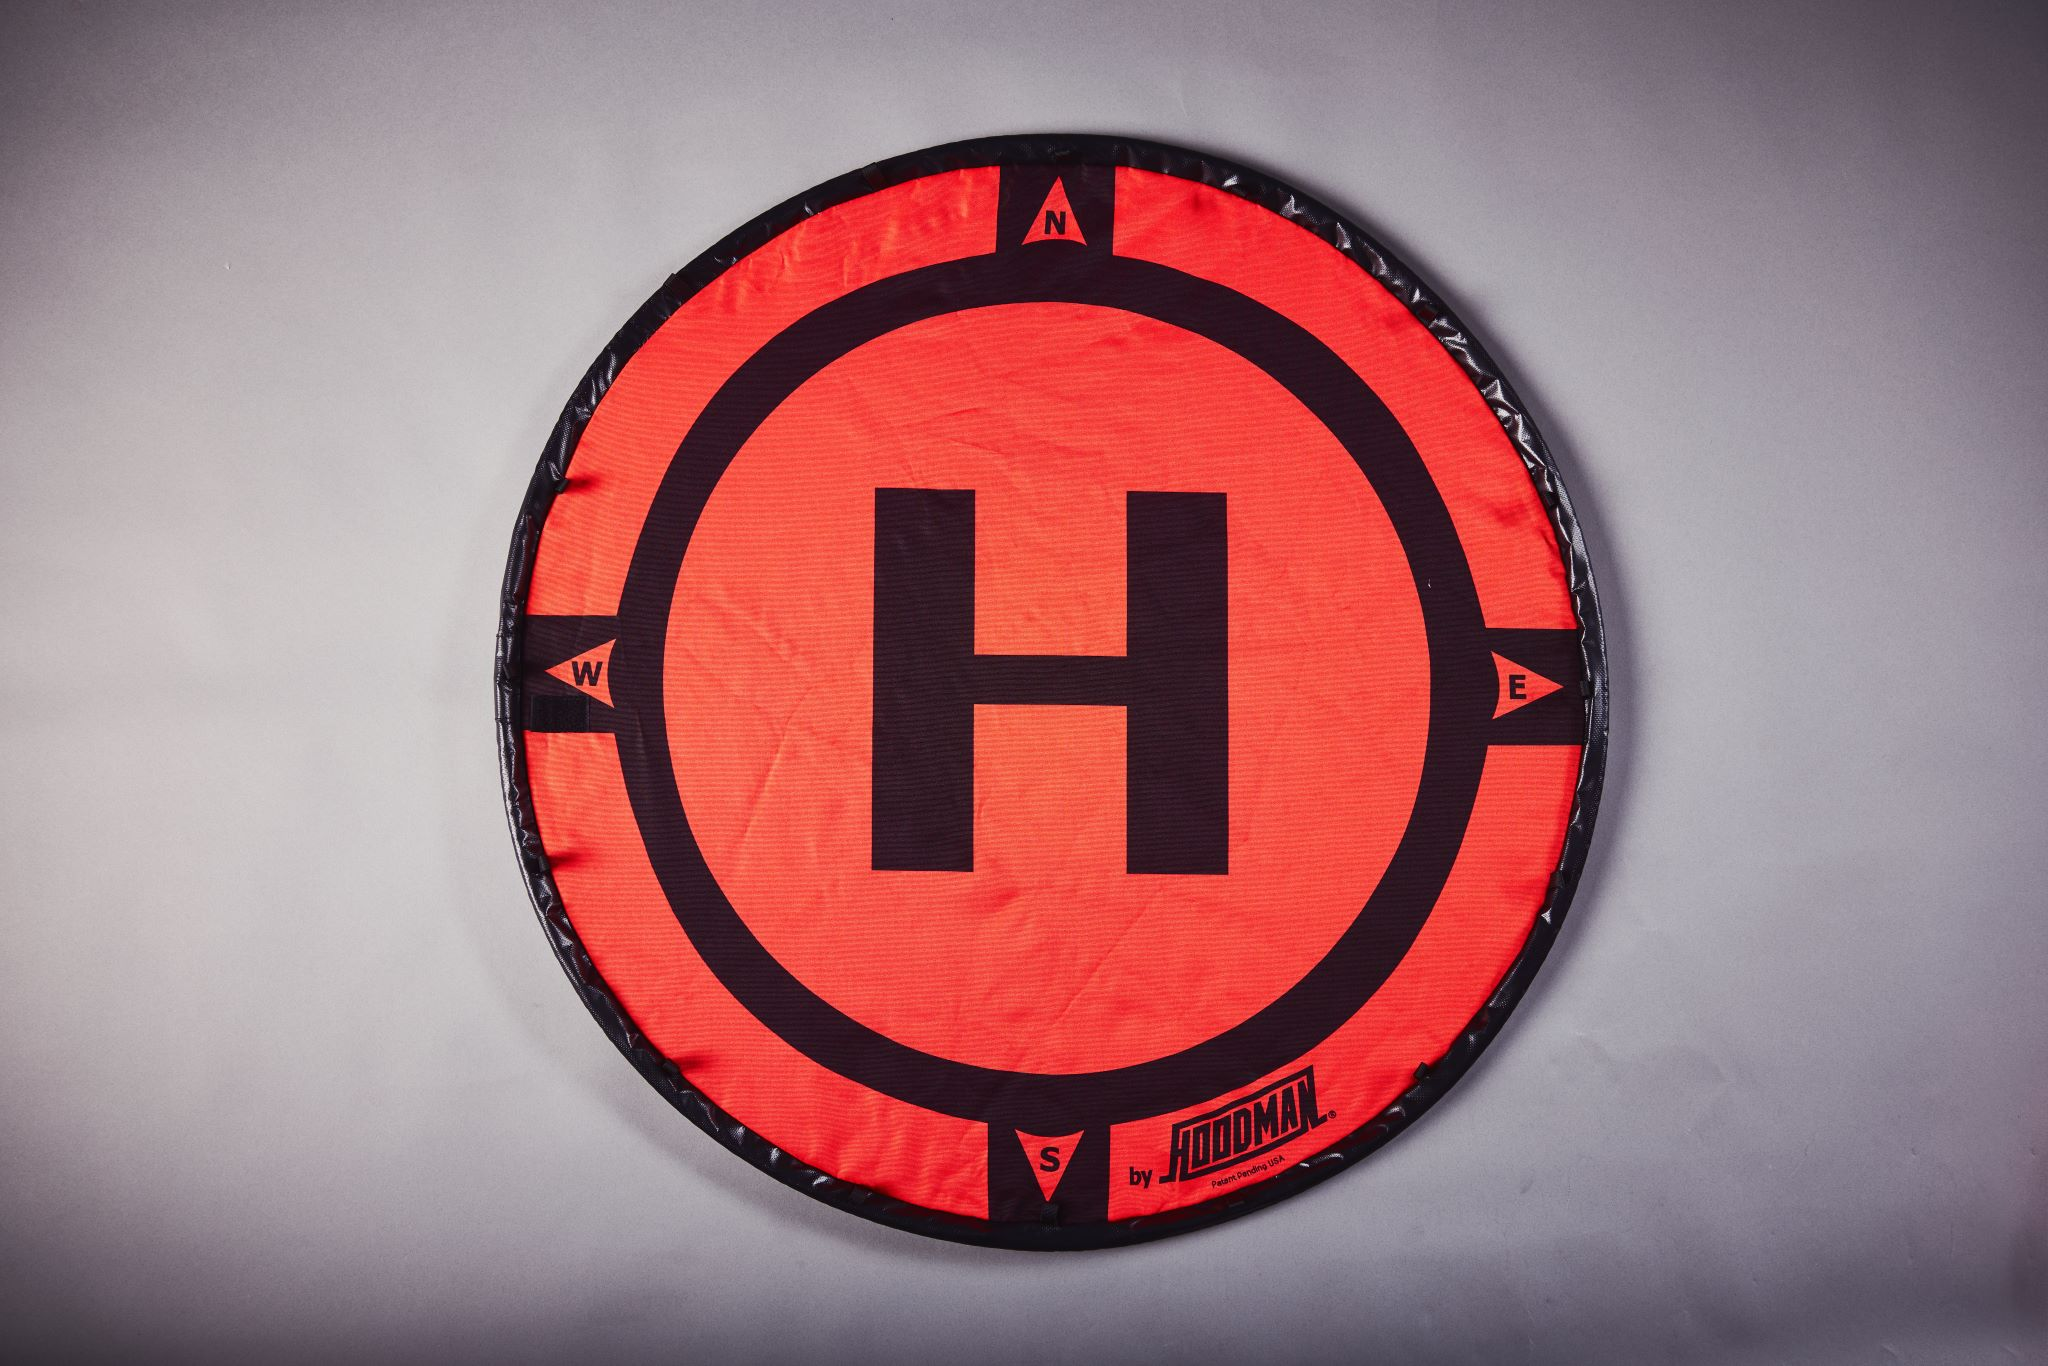
\includegraphics[height=4cm, keepaspectratio]{general_landing_pad.jpg}
    \caption{Generic landing pad used in this work.}
    \label{fig:landingpad}
\end{subfigure}
\caption{Comparison of marker-based and marker-less landing zone 
         identification approaches.}
\label{fig:landingcomparison}
\end{figure}

\subsection{Previous Approaches to Obstacle Detection for UAS Landing}

Previous work has attempted to tackle this issue of general obstacle detection in a couple different ways. A benchmarking study of closed-set detectors for small UAS autonomous landing~\cite{vu2025transformer} explored the tradeoff between convolutional neural networks (CNN) YOLOv8 and Real-Time Detection Transformer (RT-DETR). The study found that transformer based models such as RT-DETR are better suited for applications where it is necessary to optimize for uncertainty quantification to increase safe UAS landings, while CNNs like YOLOv8 are better for raw inference speed and real-time performance. However, both approaches remain constrained by the fundamental limitation of closed-set detection: neither can identify obstacles outside their fixed training categories.

To address this, the See\&Say \cite{ghazanfari2026seesay} framework applied cloud-based vision-language models to identify safe vs unsafe landing zones and even propose alternative landing zones should the landing pad be occupied. While See\&Say offers very promising results, it is not explicitly designed for real-time operation due to latency from VLM inference and external API communication. In practice, this model could be run periodically (e.g., every 15 seconds) in order to obtain a general understanding of the environment but would require a lighter but faster model to run in parallel just in case there is a major change to the environment between runs, such as a child running into frame or a car pulling into the driveway. This work directly addresses that limitation by fine-tuning YOLO-World for open-vocabulary obstruction detection at real-time inference speeds on embedded Jetson hardware, enabling continuous per-frame monitoring without cloud dependency.


\subsection{Open-Vocabulary Object Detection}

The inability of closed-set detectors to recognize categories 
outside their training distribution motivates the use of 
Open-Vocabulary Object Detection (OVOD), which associates visual 
regions with arbitrary natural language descriptions rather 
than a fixed label set. CLIP~\cite{radford2021learning} 
demonstrates that rich visual representations can be learned 
by aligning image and text embeddings across 400 million 
image-text pairs collected from the internet. By encoding a 
category name as a text prompt and comparing it against image 
embeddings at inference time, the model can recognize visual 
concepts it was never explicitly trained to classify. A recent survey for OVOD in UAS Imagery~\cite{zhou2025ovuavsurvey} identifies {CLIP} as a critical breakthrough that significantly enhances aerial scene understanding and offers a very promising path forwards for future research. While this work focuses on {YOLO-World}, other {CLIP}-based {OVOD} approaches have also been explored 
for aerial detection, including {CLIP}-activated student-teacher learning~\cite{li2024clipaerial} and pseudo-label-based vocabulary expansion~\cite{li2024castdet}.

Early open-vocab object detectors, such as OVR-CNN, achieved strong generalization but carried significant computation overhead, relying on large transformer-based architectures and online vocabulary processing that made real-time deployment impractical on resource-constrained hardware \cite{zareian2021ovrcnn, cheng2024yoloworld}. YOLO-World addressed this by integrating a CLIP-based text encoder into the real-time YOLO framework and introducing a Re-parameterizable Vision-Language Path Aggregation Network 
(RepVL-PAN), illustrated in Fig.~\ref{fig:yoloworldarch}.  Its prompt-then-detect paradigm encodes the user vocabulary offline and re-parameterizes it into convolutional weights before inference, eliminating the per-image text encoding cost that bottlenecked earlier open-vocabulary detectors \cite{cheng2024yoloworld}. A further capability relevant to this work is YOLO-World's ability to respond to descriptive noun phrases. Prompts such as "person in red" or "the tallest person", allow users to specify target categories through rich natural language descriptions rather than single-word class labels. This property is particularly valuable for UAS landing obstruction detection, where general descriptive prompts such as "foreign object on orange circle landing pad" may capture hazards that would not be identified by any fixed class label.

\begin{figure}[hbt!]
\centering
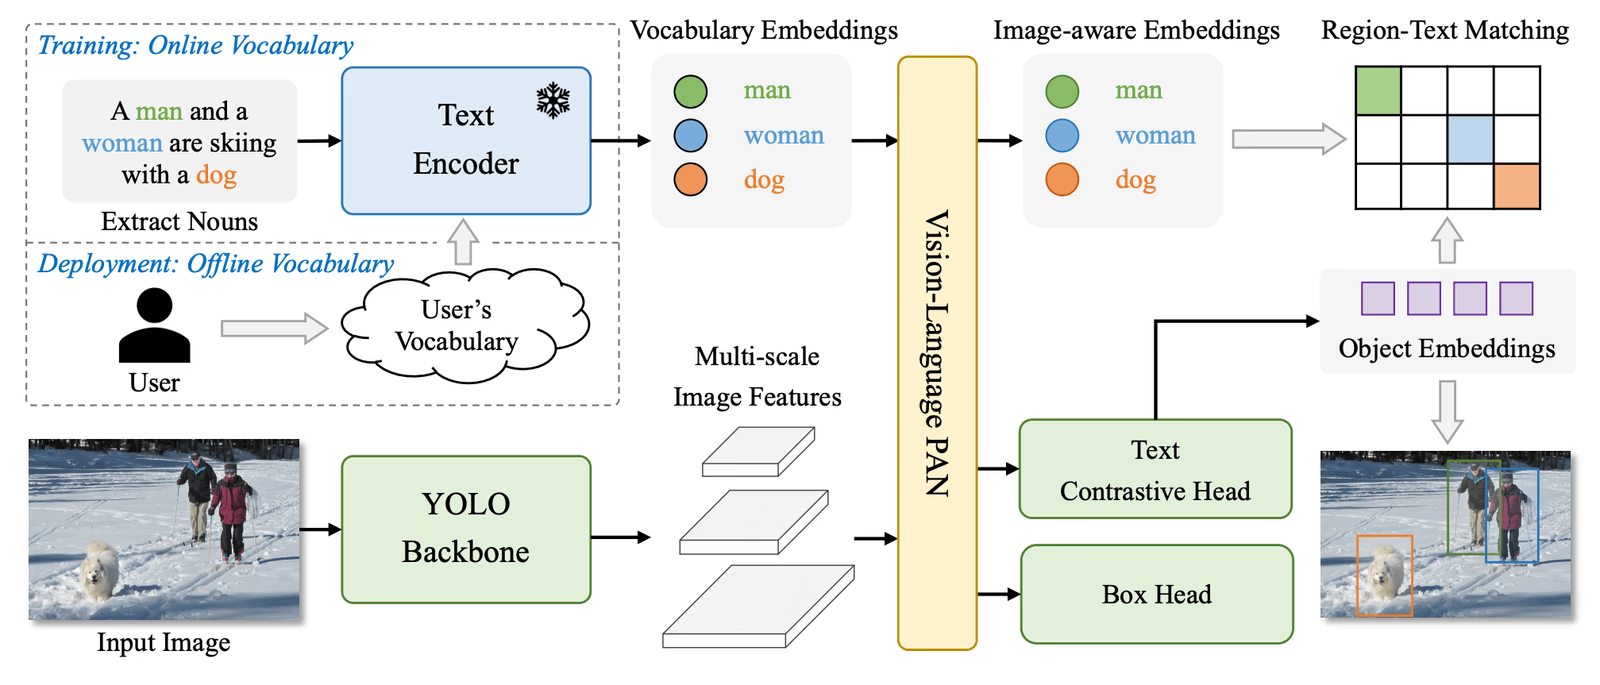
\includegraphics[width=0.95\textwidth]{yolo_world_architecture_breakdown.png}
\caption{YOLO-World architecture. The CLIP text encoder processes user-defined 
         text prompts into offline vocabulary embeddings, which are fused with 
         multi-scale image features via the Re-parameterizable Vision-Language 
         Path Aggregation Network (RepVL-PAN) to produce open-vocabulary 
         detection outputs \cite{cheng2024yoloworld}.}
\label{fig:yoloworldarch}
\end{figure}

\subsection{Fine-Tuning Open-Vocabulary Models for Aerial Domains}

The vast majority of images used to pre-train models such as YOLO-World and CLIP are captured from ground-level perspectives, creating a domain gap when deployed on UAS systems that capture top-down imagery. Pedestrians appear as small indistinct shapes, vehicles lose their distinguishing features, and spatial relationships change fundamentally, motivating domain-specific fine-tuning on aerial datasets such as VisDrone \cite{zhu2021detection}.

Fine-tuning on domain-specific data, however, risks degrading general capabilities acquired during large-scale pretraining, a phenomenon known as catastrophic forgetting \cite{mccloskey1989catastrophic}. Fine-tuning the CLIP text encoder is shown to lead to a severe drop in zero-shot generalization and it is recommended to use a reduced learning rate on the encoder as a partial mitigation \cite{cheng2024yoloworld}. Alternatively, the YOLO-IOD framework~\cite{zhang2026yoloiodrealtimeincremental} proposes 
selective kernel fine-tuning and asymmetric knowledge distillation to prevent forgetting when adding new closed-set classes sequentially. However, YOLO-IOD targets closed-set class expansion rather than open-vocabulary retention and requires significant architectural modifications. This work instead prevents encoder degradation by freezing the {CLIP} text encoder 
weights throughout fine-tuning.

\section{Methodology}

This section describes the experimental methodology for 
fine-tuning YOLO-World on the VisDrone aerial dataset 
while preserving open-vocabulary generalization. The {CLIP} 
text encoder is fully frozen throughout training, 
restricting weight updates to the detection head and neck 
to protect the pretrained visual-semantic alignment 
responsible for zero-shot detection. Three fine-tuning 
durations, 5, 40, and 80 epochs, are evaluated using a 
dual-dataset framework measuring both VisDrone domain 
accuracy and open-vocabulary retention on a custom 
Open-Vocabulary Benchmark (OVB), empirically characterizing 
the specialization-retention tradeoff as training progresses.

\subsection{Base Model}

All experiments are initialized from the pretrained YOLO-World v2 Medium (YOLOv8m-WorldV2) checkpoint, which provides a strong balance between detection accuracy and inference speed suitable for embedded deployment. 

\subsection{Dataset Preparation}

Fine-tuning is performed on the VisDrone-DET2019 dataset, a large-scale aerial imagery benchmark comprising 10,209 drone-captured images across 10 object categories: pedestrian, people, bicycle, car, van, truck, tricycle, awning-tricycle, bus, and motor \cite{zhu2021detection}. The dataset is split into 6,471 training images and 548 validation images. 

VisDrone annotations are provided in a custom text format that is incompatible with the COCO JSON format required by the Ultralytics YOLO-World training pipeline. A conversion script was developed to transform the VisDrone annotations into COCO-compatible JSON, mapping each of the 10 VisDrone class labels to sequential integer indices. A configuration file was constructed, required by the Ultralytics \cite{ultralytics2023} training framework to initialize the detection head with the correct output dimensions.

\subsection{CLIP Encoder Freezing Strategy}

The central design decision of the fine-tuning strategy is freezing the CLIP text encoder's weights and restricting weight updates exclusively to the detection head and neck. This preserves the text-image alignment responsible for zero-shot generalization while allowing the visual detection components to adapt to the aerial imaging characteristics of the VisDrone dataset. 

\subsection{Open-Vocabulary Benchmark (OVB) Evaluation Dataset}

To validate that our fine-tuning approach preserves the model's open-vocabulary capabilities, we construct an Open-Vocabulary Benchmark (OVB) evaluation set. OVB consists of 195 images that were curated using our own UAS and manually annotated with object categories that were deliberately excluded from the fine-tuning process. These categories consisted of basic obstructions (soccer ball, orange circle landing pad, dog) and descriptive noun phrases (foreign object on orange circle landing pad, foreign object on driveway). 

\subsection{Training Durations}

To monitor the progression of open-vocabulary capability 
degradation during fine-tuning, we train for three distinct 
durations: 5, 40, and 80 epochs. All three runs use 
identical hyperparameters, summarized in 
Table~\ref{tab:hyperparams}, differing only in total 
training duration. Performance is assessed using a 
dual-dataset evaluation framework, measuring both VisDrone 
mAP on the VisDrone validation set and OVB mAP on the OVB 
dataset simultaneously, an approach analogous to the 
dual-task evaluation employed by a fine-tuning 
study~\cite{gandhi2025finetuningforgettingadaptationyolov8} 
and the base/novel class evaluation protocol established 
in open-vocabulary detection 
literature.\cite{zareian2021ovrcnn}


\begin{table}[hbt!]
\caption{Fine-tuning hyperparameters. All three training runs
       (5, 40, and 80 epochs) use identical settings, differing
       only in total training duration.}
\label{tab:hyperparams}
\centering
\begin{tabular}{ll}
\hline
\textbf{Parameter} & \textbf{Value} \\
\hline
Base model          & YOLOv8m-WorldV2 \\
Optimizer           & AdamW (auto) \\
Learning rate (lr0) & $2 \times 10^{-4}$ \\
LR decay (lrf)      & 0.01 \\
Weight decay        & 0.05 \\
Batch size          & 24 \\
Image size          & $1280 \times 1280$ \\
Warmup epochs       & 3 \\
\hline
\end{tabular}
\end{table}

\section{Results}

\subsection{Quantitative Results}

Table~\ref{tab:results} summarizes performance across all checkpoints. VisDrone mAP and OVB mAP average IoU thresholds from 0.5 to 0.95 on the VisDrone validation set and OVB set, respectively.

\begin{table}[hbt!]
\caption{Performance comparison across fine-tuning checkpoints on 
         VisDrone validation and Open-Vocabulary Benchmark sets.}
\label{tab:results}
\centering
\begin{tabular}{lccc}
\hline
\textbf{Model} & \textbf{VisDrone mAP} & \textbf{VisDrone mAP@50} 
& \textbf{OVB mAP} \\
\hline
Base (YOLOv8m-WorldV2) & 0.131 & 0.198 & 0.034 \\
Fine-tuned (5 epoch)   & 0.308 & 0.492 & 0.034 \\
Fine-tuned (40 epoch)  & 0.298 & 0.476 & 0.017 \\
Fine-tuned (80 epoch)  & 0.330 & 0.525 & 0.001 \\
\hline
\end{tabular}
\end{table}

Fine-tuning on the VisDrone dataset produces substantial 
gains in domain-specific detection accuracy across all 
checkpoints. The 5-epoch checkpoint achieves a VisDrone 
mAP of 0.308, representing a +135\% improvement over the 
base model, and a mAP@50 of 0.492, a +149\% improvement. 
The slight mAP decrease from 5 to 40 epochs (0.308 
vs.\ 0.298) is attributable to training variance, as the 
80-epoch checkpoint recovers to 0.330, confirming that 
VisDrone accuracy does not monotonically decline with 
training duration. Per-class results in 
Table~\ref{tab:perclass} show consistent improvement 
across all 10 VisDrone categories, with the most 
notable gain on the motor class, which improves from 
0.000 in the base model to 0.303 after fine-tuning, 
indicating that zero-shot detection of certain aerial 
categories fails entirely without domain adaptation.

The OVB mAP results reveal a clear and consistent 
pattern of open-vocabulary capability loss with extended 
fine-tuning. The 5-epoch checkpoint retains an OVB mAP 
of 0.034, identical to the base model baseline, 
indicating that 5 epochs of frozen-encoder fine-tuning 
produces no measurable degradation in open-vocabulary 
detection accuracy. In contrast, the 40-epoch checkpoint 
degrades to an OVB mAP of 0.017, a 49\% reduction 
relative to baseline, and the 80-epoch checkpoint 
collapses to near zero at 0.001.


\begin{table}[hbt!]
\caption{Per-class AP on VisDrone validation set 
         (COCO mAP@[.5:.95]).}
\label{tab:perclass}
\centering
\begin{tabular}{lcc|lcc}
\hline
\textbf{Class} & \textbf{Base} & \textbf{5-epoch} & 
\textbf{Class} & \textbf{Base} & \textbf{5-epoch} \\
\hline
pedestrian      & 0.081 & 0.325 & truck           & 0.156 & 0.338 \\
people          & 0.044 & 0.215 & tricycle        & 0.023 & 0.230 \\
bicycle         & 0.064 & 0.155 & awning-tricycle & 0.036 & 0.123 \\
car             & 0.469 & 0.622 & bus             & 0.293 & 0.454 \\
van             & 0.149 & 0.317 & motor           & 0.000 & 0.303 \\
\hline
\end{tabular}
\end{table}

\subsection{Embedded Deployment}

The 5-epoch fine-tuned checkpoint was evaluated for real-time inference on two embedded platforms: the Jetson Xavier and the Jetson Orin Nano. Embedded inference on {NVIDIA} Jetson platforms has been 
demonstrated across a range of real-time computer vision 
tasks, with the Jetson ecosystem providing a practical 
deployment target for {UAS} onboard 
computing \cite{mittal2019survey}. Inference was performed at 1280$\times$1280 resolution using the PyTorch runtime. Table~\ref{tab:jetson} summarizes the measured inference speeds across both platforms.

\begin{table}[hbt!]
\caption{Real-time inference performance of the 5-epoch 
         fine-tuned checkpoint on embedded Jetson platforms 
         at 1280$\times$1280 resolution.}
\label{tab:jetson}
\centering
\begin{tabular}{lccc}
\hline
\textbf{Platform} & \textbf{FPS}  \\
\hline
NVIDIA Jetson Xavier      & 9.4 \\
NVIDIA Jetson Orin Nano & 12.5  \\
\hline
\end{tabular}
\end{table}

Both platforms sustain real-time inference speeds suitable for onboard UAS deployment, confirming that the fine-tuned 
open-vocabulary detection system is practical for resource-constrained aerial hardware, and suggest that performance can be further improved via more powerful embedded systems such as NVIDIA Jetson Thor.

\begin{figure}[hbt!]
\centering
\begin{subfigure}{0.45\textwidth}
    \centering
    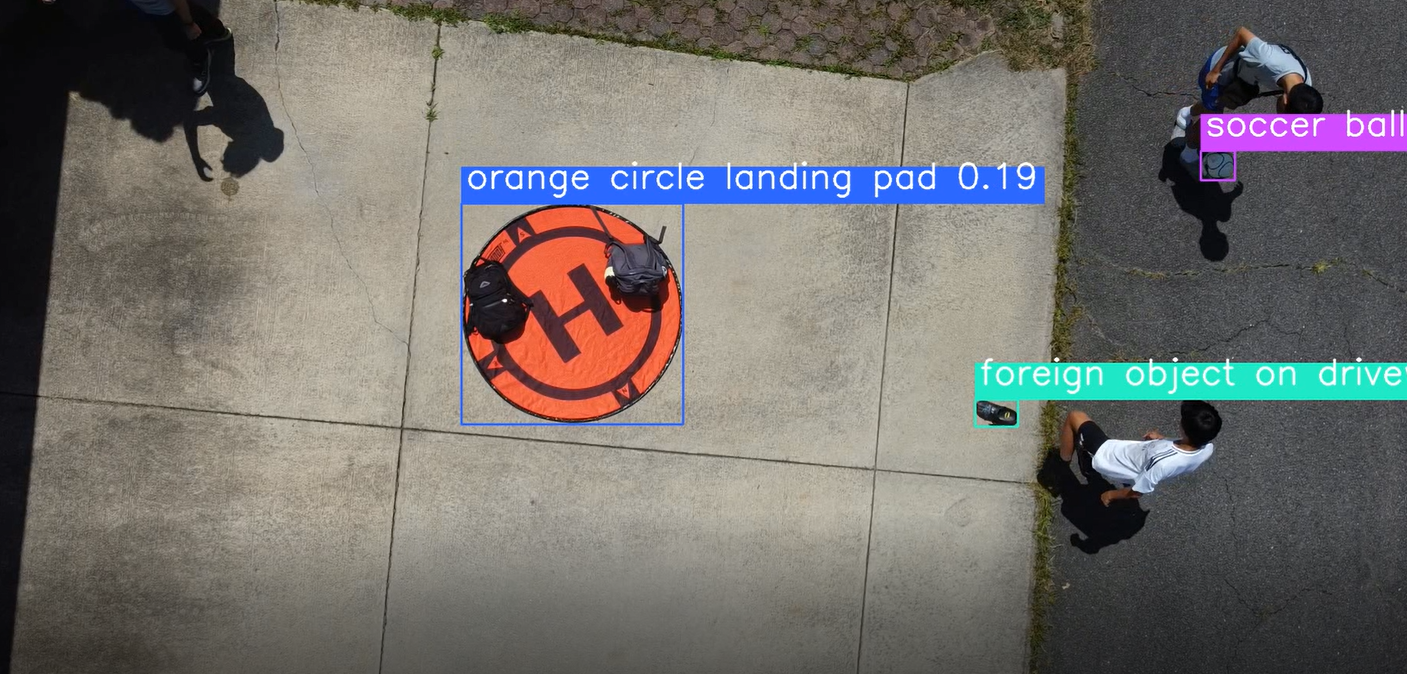
\includegraphics[height=4cm, keepaspectratio]{baseline_4.png}
    \caption{Base YOLOv8m-WorldV2 model.}
    \label{fig:pedestrian_base}
\end{subfigure}
\hfill
\begin{subfigure}{0.45\textwidth}
    \centering
    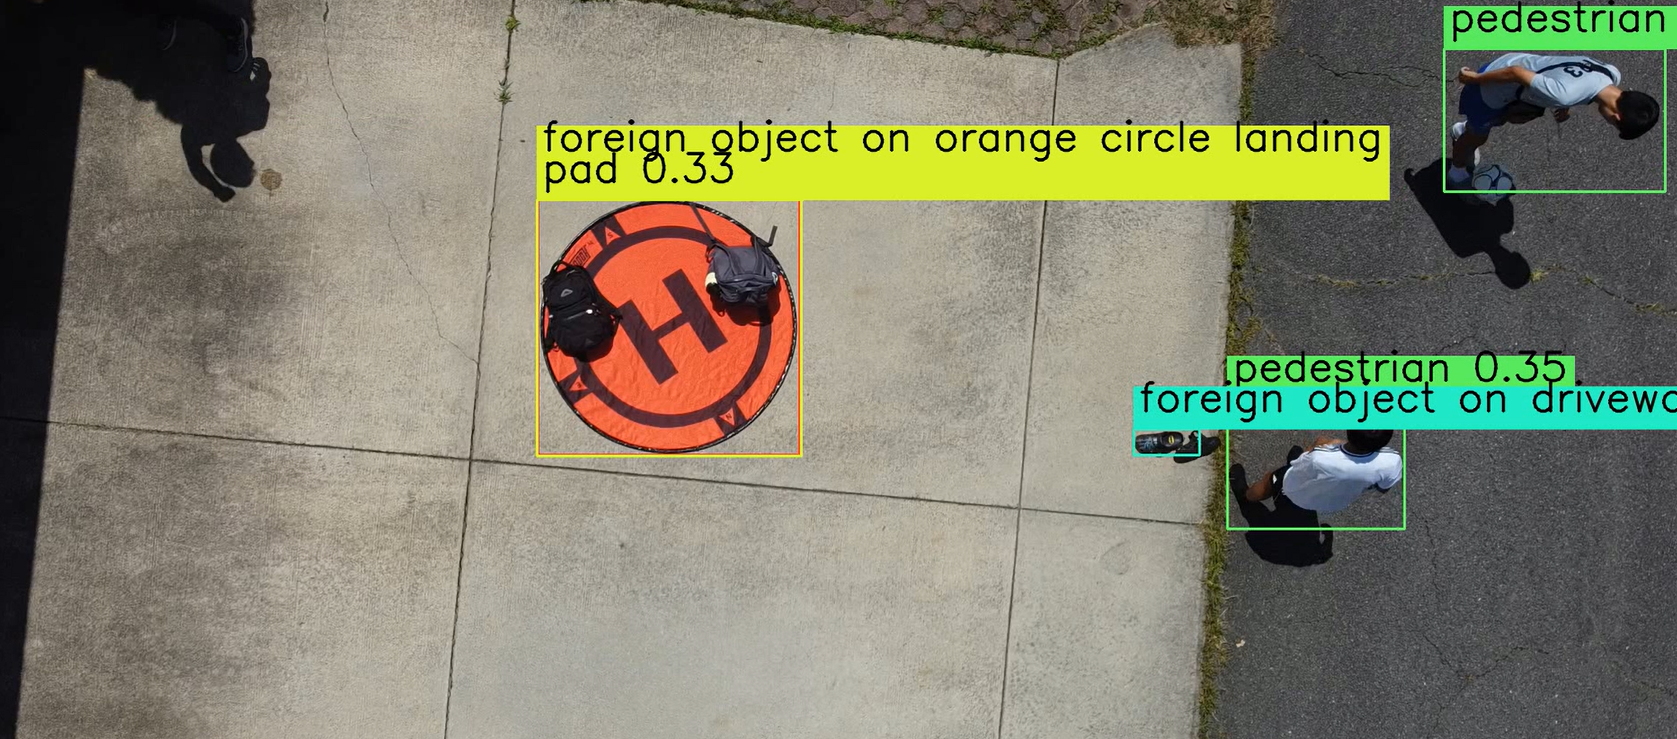
\includegraphics[height=4cm, keepaspectratio]{finetuned_4.png}
    \caption{Fine-tuned (5 epoch).}
    \label{fig:pedestrian_ft}
\end{subfigure}
\caption{Base model (left) vs.\ 5-epoch fine-tuned model (right) 
         on top-down pedestrian detection.}
\label{fig:pedestrian_comparison}
\end{figure}

\begin{figure}[hbt!]
\centering
\begin{subfigure}{0.45\textwidth}
    \centering
    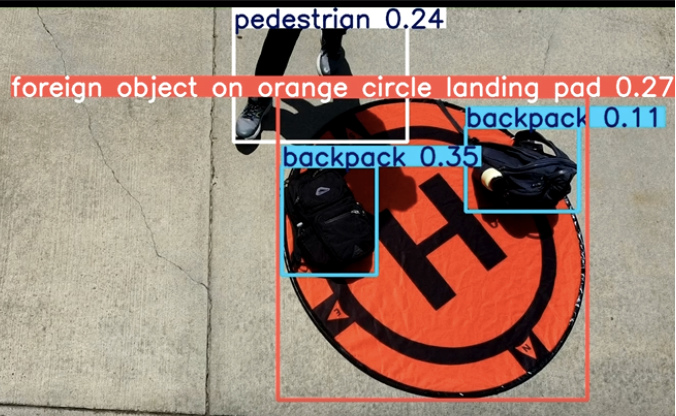
\includegraphics[height=4cm, keepaspectratio]{landing_pad_backpack_before_ov_loss.png}
    \caption{Base YOLOv8m-WorldV2 model.}
    \label{fig:backpack_base}
\end{subfigure}
\hfill
\begin{subfigure}{0.45\textwidth}
    \centering
    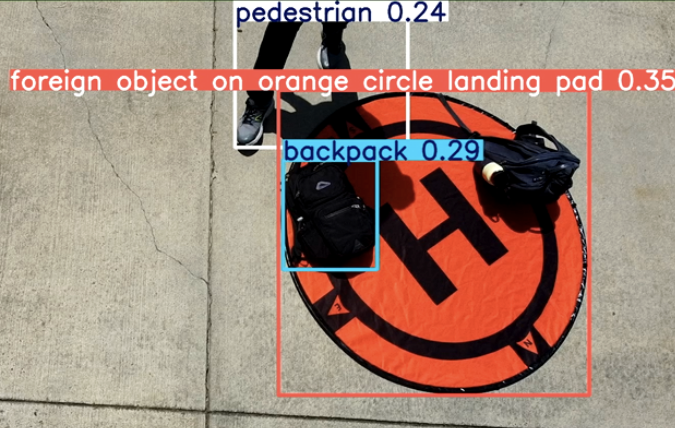
\includegraphics[height=4cm, keepaspectratio]{landing_pad_backpack_after_ov_loss.png}
    \caption{Fine-tuned (5 epoch).}
    \label{fig:backpack_ft}
\end{subfigure}
\caption{Base model (left) vs.\ 5-epoch fine-tuned model (right). 
         Even short fine-tuning durations reduce detection confidence 
         on open-vocabulary classes outside the VisDrone distribution.}
\label{fig:backpack_comparison}
\end{figure}

\section{Discussion}

The results reveal a clear tradeoff between domain specialization and open-vocabulary retention as fine-tuning duration increases. Despite the CLIP encoder being fully frozen throughout training, 
open-vocabulary capability degrades rapidly beyond 5 epochs, suggesting that the detection head and neck progressively bias toward VisDrone classes regardless of our attempts to mitigate this. Fig. \ref{fig:backpack_comparison} demonstrates this problem clearly, showing the confidence and detection accuracy on the prompted OVB class "backpack" decreases with finetuning. The 5-epoch checkpoint represents the most practical configuration, achieving +135\% VisDrone mAP improvement while retaining OVB mAP at baseline levels, as demonstrated qualitatively in Fig.~\ref{fig:pedestrian_comparison} where the detection on VisDrone classes, such as "pedestrian", has improved dramatically at the cost of prompted open-vocab classes such as "soccer ball".

Several limitations bound these findings. The 195-image OVB set is sufficient to establish trends but too small for statistically robust mAP estimates. Only three epoch checkpoints at a fixed learning rate were evaluated, while a systematic hyperparameter search or experiments with partial freezing of the CLIP encoder may yield a more favorable tradeoff than identified here. 

A practical limitation of this approach is that target classes must be prompted before inference, requiring prior knowledge of potential obstructions. This can be partially addressed using an exhaustive prompt list of common hazard categories and the descriptive prompts to catch more obscure "foreign obstacles". Future work will explore using vision-language models, either cloud-based or compact onboard models such as LiteVLM \cite{huang2025litevlmlowlatencyvisionlanguagemodel}, to dynamically generate prompts from a scene prior to YOLO-World inference, eliminating the need for manual prompt specification.

\section{Expected Outcomes}

Prior to final submission, additional experiments will be conducted to further investigate open-vocabulary retention during fine-tuning. Planned approaches include lower learning rates, which online resources suggest may reduce capability degradation, as well as partial freezing of specific CLIP encoder layers or training a separate detection head as alternative mitigation strategies \cite{gandhi2025finetuningforgettingadaptationyolov8}.

Additionally, evaluation will be extended to the LVIS dataset, the benchmark used in the original YOLO-World evaluation, to provide a standardized measure of open-vocabulary degradation relative to the pretrained baseline independent of the OVB set \cite{cheng2024yoloworld}. We will also compare our results with previous work on closed set detectors using YOLOv8 and RT-DETR~\cite{vu2025transformer}.

\section{Conclusion}

This paper presented a fine-tuning methodology for adapting YOLO-World to UAS landing zone obstruction detection and explored the trade-off between VisDrone domain specific accuracy and open vocabulary retention. We demonstrate that open-vocabulary capability collapses rapidly with extended training even under encoder protection. This proves that while freezing the CLIP encoder mitigates the damage, on its own it isn't enough to fully preserve open vocabulary capability. The 5-epoch checkpoint achieves the strongest balance between VisDrone accuracy and open-vocabulary retention, capable of using descriptive noun phrase prompts to detect novel obstructions at inference time, and real-time performance is confirmed on NVIDIA Jetson Xavier and Jetson Orin Nano platforms. These results establish a practical foundation for open-vocabulary obstruction detection in autonomous UAS landing and motivate future work on retention-aware fine-tuning strategies and dynamic prompt generation via vision-language model integration.

% \section*{Acknowledgments}

% ...

\bibliography{sample}
% \bibliographystyle{aiaa}  % new-aiaa.cls already sets new-aiaa; a second style makes BibTeX error


\end{document}